\documentclass[english,12pt]{article}
\usepackage{wrapfig}
\usepackage{float}
\usepackage[english]{babel}
\usepackage[utf8]{inputenc}
\usepackage[T1]{fontenc}
\usepackage{hyperref}
\usepackage{siunitx}
\usepackage{graphicx}
\usepackage{gensymb}
\usepackage{tabularx}
\usepackage{longtable}
\usepackage{sidecap}
\usepackage[normalem]{ulem}
\useunder{\uline}{\ul}{}
\usepackage[hmargin=1in,vmargin=1in]{geometry}
\usepackage[dvipsnames]{xcolor}
\usepackage[normalem]{ulem}
\usepackage{flafter} 
\usepackage[section]{placeins}
\useunder{\uline}{\ul}{}
\begin{document}

\begin{center}

\thispagestyle{empty}

$ $

\vspace{250pt}

\begin{bfseries}

{\Large Object Recognition and Path Smoothing Robot, Phase 6}

{\Huge Design Specification}

%{\Large $\langle$application and version to be tested$\rangle$}%

\end{bfseries}

\vspace{180pt}

University of Washington Tacoma, School of Engineering and Technology

%TIE-21204 Ohjelmistojen testaus%

\vspace{12pt}

Authors: 

Ammon Dodson \href{mailto:ammon0@uw.edu}{ammon0@uw.edu} 

Alex Marlow \href{mailto:alexmarlow117@gmail.com}{alexmarlow117@gmail.com} 

Jake McKenzie \href{mailto:jake314@uw.edu}{jake314@uw.edu}

Distribution: Matthew Tolentino

Document state: draft

Modified: \today

\end{center}

\newpage


\tableofcontents

\newpage


\section{Revision History}

\begin{itemize}
	\item v0.1.0: Initial specifications for the document itself.
    \item v0.2.0: Additional information was added about the Robot 
    Operating System (ROS).
    \item v0.2.1: Ethical concerns were added to the document.
    \item v0.2.2: Created a diagram for the overall system architecture.
    \item v0.3.0: Additions to the introduction. Rewrite of the requirements section with
    enumeration. Additions to the System Architecture and System Design
    section including hardware architecture and software architecture with
    higher level and lower level diagrams with text describing these diagrams
    and text for these sections generally.
    \item v0.4.0: Made the requirements table. Clarified some requirements. Improved page
    formatting. Added some to the design section. Use case diagram created for
    the introduction and general mistakes addressed.
    \item v0.5.0: The entire document was ported from microsoft word to LATEX.
    A paragraph worth of text was removed and what was left was refined to be more direct 
    as to what we were doing focusing on one question. Communication protocol was established.
    Document wording was refined to only talk about the researchers name when applicable.
    All instances in the architecture section that mentioned specific hardware have been 
    removed from the architecture section and the design section has been fleshed out more.
    Objectives were added to software design and every architecture section had all instances to 
    specific devices removed. A new diagram was reworked in hardware architecture to remove all 
    instances of specific hardware.
    \item v0.6.0 cake diagram in software architecture was added
\end{itemize}
\newpage
\section{Introduction}
\subsection{Overview}
\FloatBarrier
\begin{figure}[H]
    \centerline{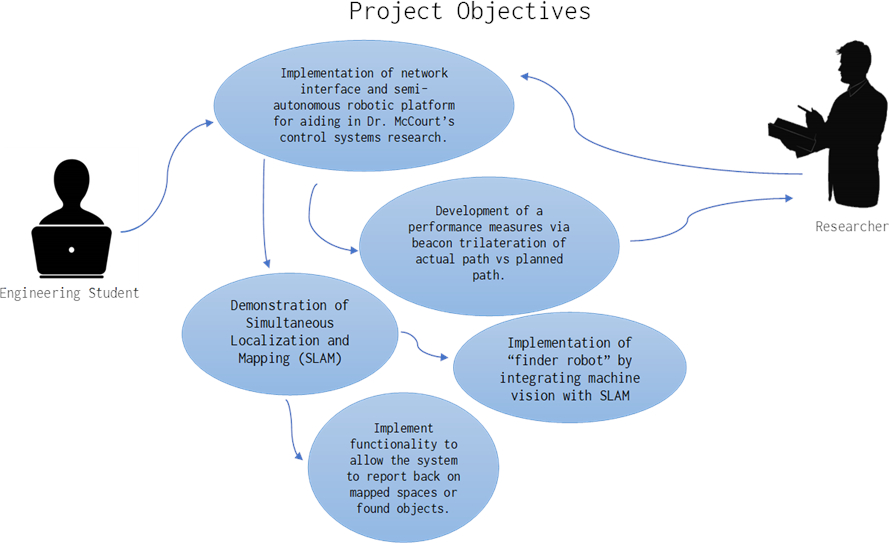
\includegraphics[width = \textwidth]{proj_obj.jpg}}
    \caption{Use case diagram for the overall project}
\end{figure}
\FloatBarrier
This design specification describes the architectures and design framework that will aid and abet the
production of the ORPS-Robot – The Object Recognition and Path Smoothing Robot. The
ORPS-Robot will be a platform for validating the research of Michael McCourt and a scheme for
exploring object recognition via OpenCV with Robot Operating System, which is a powerful framework
for writing robot software, with a demonstration of Simultaneous Localization and Mapping
(SLAM). Together this will demonstrate a “finder robot” with applications in search and rescue and
threat detection.\\\\
The project aims
at investigating the dynamics of a semi-autonomous robot with the 
ORPS-Robot by delivering a platform that is some interplay of communications, computing and
software to aid in research in control.
Essentially this project aims at reducing the negative effects of controlling a system over 
some communication delay by delivering a framework that can be used in a generic way by 
an algorithm developed for smoothing outputs to some system, reducing uncertainty and 
providing a smooth experience that users expect when using devices. This involves building 
a framework not only for testing the algorithm but collecting data for use in a simulator 
for further optimization and validation.

\subsection{Network Control}
\begin{wrapfigure}{r}{0.4\textwidth}
    \begin{center}
      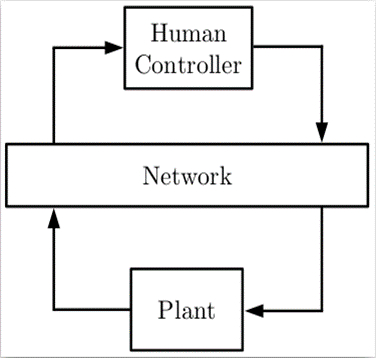
\includegraphics[width=0.38\textwidth]{typ_cs.jpg}
    \end{center}
    \caption{A typical networked control system}
  \end{wrapfigure}
Network control systems have many useful applications; The typical use case involves using robots to
interact with an environment that is too hazardous for a person. Any such Network control involves
some delay of both outgoing control signals and incoming sensor data. In some situations, this delay
may impair the intended function of the network control system.\\\\
A set of input/output transformation algorithm have been developed and are
 intended to be placed in such a delayed, closed-loop control
system. These filters apply a mathematical transformation on both incoming and outgoing loop signals
such that communication delays are mitigated. This specification outlines the development of a
controller-robot system intended to demonstrate the algorithm.
\subsection{Autonomous Control}
There may also be use cases for robots in hazardous environments where direct human control is
impossible. Such a robot must be able to autonomously navigate and interact with an unknown space.
SLAM is a fundamental technology for such autonomous activity, allowing the robot to navigate.
Additionally, such an autonomous machine must be able to sense and recognize an objective before
being able to interact with it. Computer vision is another
fundamental technology for sensing a real-world environment.
Sensing a condition is a necessary first step for being able to act
based on the current environment.
\subsection{Scope}
This specification covers the following:\\
\begin{itemize}
    \item Any and all hardware modifications to the ORPS-Robot.
    \item Software installed on the burger bot insofar as it deviates
    from the stock installation.
    \item Base station control software setup insofar as it deviates
    from stock installation.
    \item Any necessary techniques for integrating a Human
    Interface to the base station installation.
    \item Any methods used to implement a communication delay
    between the robot and its base station.
    \item Implementation of the input output transformation.
    \item An overview of implementing SLAM on the ORPS-Robot.
    \item Integration of OpenCV into the ORPS-Robot.
\end{itemize}
\section{Requirements}
In this section we will delve through the minimum requirements of this project to translate the needs of
our client Michael McCourt into precise targets, establish metrics for a successful product and support
design trade-off decisions. For this revision of the design specification we will articulate the marginally
acceptable target values, without any of the ideal target values for our stretch goals.
\begin{table}[ht]
\begin{tabular}{|l|l|}
\hline
Requirement Number & Requirement Criteria \\ \hline
R1 & There must exist a mobile platform \\ \hline
R2 & \begin{tabular}[c]{@{}l@{}}There must be a base station \\ with a human interface device\end{tabular} \\ \hline
R3 & \begin{tabular}[c]{@{}l@{}}The base station must communicate \\ with the mobile platform through \\ a delayed link\end{tabular} \\ \hline
R4 & \begin{tabular}[c]{@{}l@{}}The mobile platform must be \\ wirelessly controllable\end{tabular} \\ \hline
R5 & \begin{tabular}[c]{@{}l@{}}The mobile platform must be \\ able to report its position \\ in space\end{tabular} \\ \hline
R6 & \begin{tabular}[c]{@{}l@{}}There must be a means of \\ recording and comparing \\ the planned and actual path\end{tabular} \\ \hline
R7 & \begin{tabular}[c]{@{}l@{}}The mobile platform must \\ be able to explore an unknown \\ area\end{tabular} \\ \hline
R8 & \begin{tabular}[c]{@{}l@{}}The mobile platform must \\ be able to map the unknown \\ area\end{tabular} \\ \hline
R9 & \begin{tabular}[c]{@{}l@{}}The mobile platform must \\ be able to identify and \\ locate objects in the \\ unknown area\end{tabular} \\ \hline
\end{tabular}
\end{table}
\subsection{Network Control}
\begin{itemize}
    \item[R1.] \textit{\textbf{There will be some ROS capable mobile platform.}} \\
    This robot must be ROS capable, mobile, and remotely controllable. The mobile platform must be
    capable of processing the R-transform for incoming and outgoing signals. All the hardware and software
    modules of the mobile platform must fit within the constraints of that platform, including such things as
    power, weight, and processing speed.
    \item[R2.] \textit{\textbf{There must be a base station interfaced with a USB game controller.}} \\
    The Human controller we have available currently is a USB game controller. This controller will have to
    be connected to some base station that can connect to the ORPS-Robot wirelessly. The base station is a
    laptop which will run the graphical user interface for the user, route communication traffic, perform
    transformations and public commands for the ORPS-Robot.
    \item[R3.] \textit{\textbf{The base station must communicate with the robot through a delayed link.}} \\
    In order to demonstrate the input/output transformation algorithm, the robot must be remotely
    controllable. Control signals must be routed through a delayed communication medium. Ideally, or as a
    second stage, the human controller’s feedback information should also be routed through the delayed
    medium.
    \item[R4.] \textit{\textbf{The Robot Should be wirelessly controllable.}} \\
    To fully demonstrate the usefulness of the transformation algorithm we should model a real-world situation
    where the robot is out of sight and controllable solely from the base station.
    \item[R5.] \textit{\textbf{The robot must be able to report its position in space.}} \\
    To fully demonstrate the transformation algorithm, the full control loop should be routed
    through it as shown in Figure 2. This will require the position feedback to be in the form of a simple
    numerical array such as an x-y coordinate.
    \item[R6.] \textit{\textbf{There must be a means of recording and comparing the planned and actual path the robot follows.}} \\
    To demonstrate the transformation algorithm we need to be able to compare the actual
    and planned path and have some measure of how closely they align. We should be able to make
    multiple test runs with and without the filter functioning and compare the course fidelity in aggregate.
\end{itemize}
\subsection{Autonomous Control}
\begin{itemize}
    \item[R7.] \textit{\textbf{The mobile platform should be able to explore all accessible parts of an unknown area.}} \\
    If the robot is being used to search an area it will be important to ensure that the full area has been
    searched. Otherwise the system could produce a false negative. It is also important to consider the
    orientation and effective range of any sensors to ensure that they have made adequate coverage of the
    search area. This will be accomplished by communicating with the robot, back and fourth, over WiFi with 
    communication between components being down either via USB 2.0 for most of the components and half duplex UART
    in the case of the actuators. Publishing and receiving ROS topics must be established.
    \item[R8.] \textit{\textbf{The mobile platform should be able to create a map of the area.}} \\
    In order to be useful, The map should available on the base station as quickly as possible. This map
    should also include any found objects and links to sensor data for those objects. This will require some
    sort of performance measure to be defined for both the LiDAR and Marvelmind Beacons.
    \item[R9.] \textit{\textbf{The robot should be able to identify and locate objects through computer vision.}} \\
    In order to be useful, The map should available on the base station as quickly as possible. This map
    should also include any found objects and links to sensor data for those objects. This will require some
    sort of performance measure to be deThe mobile platform should be able to be trained to identify specific objects in its environment. It should
    also be able to identify, locate, and report on the location or condition of these objects. Some sort of
    machine learning algorithm must be employed to detect objects in an environment in real time. This has
    not been well defined for our group yet and we don’t even know if we’re going to get to this portion of
    the project. This should be evident by the length of this section compared to the prior sections.fined for both the LiDAR and Marvelmind Beacons.
\end{itemize}
\section{System Architecture}

\begin{wrapfigure}{r}{0.45\textwidth}
    \vspace{-20pt}
    \begin{center}
      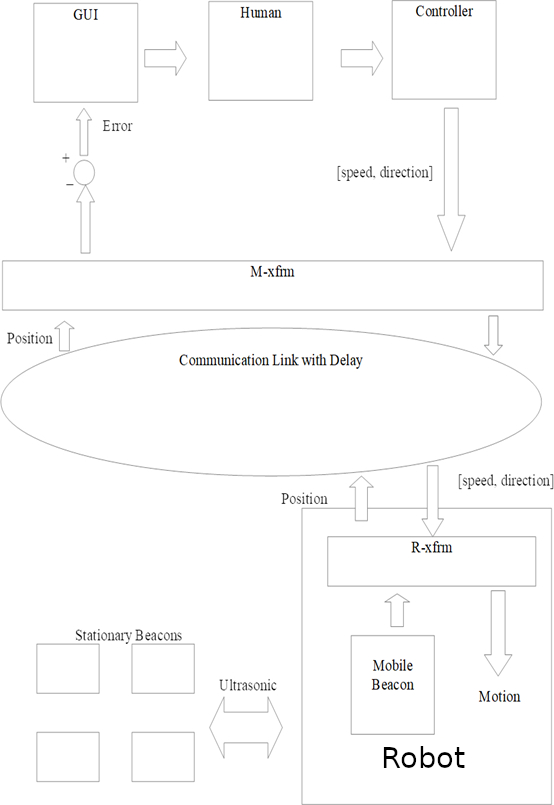
\includegraphics[width=0.43\textwidth]{sys_arc.jpg}
    \end{center}
    \vspace{-20pt}
    \caption{The System Architecture}
    \vspace{-10pt}
  \end{wrapfigure}
The main objective of ORPS-Robot (Object
Recognition and Path Smoothing) is to
validate this research
and create scheme for exploring object
recognition via OpenCV with Robot
Operating System (ROS). In this section
we will develop our methodology for the
overall system architecture by exploring
the flow of data from each component in
the overall system, by referring to the
figure 2 on our right.\\\\
First the user looks at the graphical user
interface, which displays the reported
position of the ORPS-Robot and the
desired position based on some preprogrammed
path. The user will attempt
to move the robot towards the desired
position via a controller.
Movement commands, in the form of a
vector will pass through the M-Transform
before being transmitted over Wi-Fi to
the ORPS-robot. Onboard the robot, the
control vector will pass through the R-Transform
on a single board computer before
being passed to a microcontroller as
movement commands.\\\\
Several stationary beacons will be
placed in the demonstration area. The ORPS-Robot will have mobile beacon which will
provide it with relative position information in the standard NMEA 0183 format. This data is then sent
back to the basestation via Wi-Fi going first through the R-Transform then through the M-Transform
where it is processed and presented to the user in the graphical user interface. This closes the loop. It is
worth noting that no published ROS commands on the base station or the ORPS-Robot can be sent
through the transform itself.
\subsection{Hardware Architecture}
While hardware is not the focus of this project, the
hardware architecture is an important component and
each physical component will be introduced by their
power requirements and/or communication protocols.
The main hardware components are the basestation,
ORPS-Robot and trilateralization beacons. The basestation
and ORPS-Robot will communicate via Wi-Fi while
 stationary beacons communicate amongst
themselves via ultrasonic. A mobile beacon
will communicate to a single board computer via USB 2.0. The
microcontroller will communicate to an 
actuator system via serial signal via RS-485.\\\\
On the ORPS-Robot itself a Li-Po battery feeds the
microcontroller power which will then feed the
single board computer and mobile beacon for trilateralization. The
microcontroller will be feeding power to the
actuator system for movement.\\\\
The LiDAR will be mentioned briefly but we
have not decided whether this is a crucial component
of the architecture as it is becoming a stretch goal for
the project, as such it is left out of the current set of
diagrams.
\begin{figure}
    \centerline{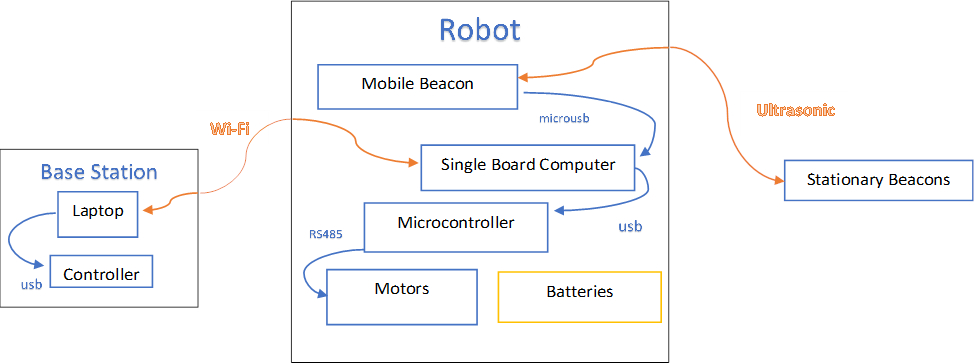
\includegraphics[scale = 1.9]{hard_arc.jpg}}
    \caption{The hardware architecture}
\end{figure}
\FloatBarrier
\subsubsection{Communication Link}
Most communications between devices in this project will be via either USB 2.0 or IEEE 802.11 Wi-Fi
apart from mobile beacons which communicates via ultrasonic amongst themselves and USB 2.0 via the
base station.
\subsubsection{ORPS-Robot}
The ORPS-Robot is a collection of disparate components meant which combine to make a semiautonomous
robot meant for validating control systems research and to serve as a vessel for
undergraduate education. The “Burger” design splits the robot into separate layers where each
component is stored. The hardware in the ORPS-Robot is a literal stack with the  LiDAR on the
top of the robot, single board computer on the middle stack and microcontroller on the bottom stack 
with the actuator system existing on the bottom with a single ball bearing for rotational
movement.
\paragraph{Single Board Computer}
Single board computer is a small computer which we are using as our main controller on the ORPS-Robot. It will be
running Linux, and act as our point of contact to the ORPS-Robot. The single board computer will be connected
to the laptop via Wi-fi, and the microcontroller and mobile beacons via USB. The single board computer will take signals
from the laptop as well as the Marvel-Mind sensors, process them, then send them to the microcontroller.
\paragraph{Microcontroller}
A controller board used for manipulating the different robotic components. This board is open
source and made specifically for working with ROS systems. This board is attached to the battery, which
it uses to supply power to all the other components on the robot. The microcontroller is attached to the
Raspberry PI 3 via USB 2.0 and to the DYNAMIXAL Actuator system via RS-485. The microcontroller is
programmable with the Arduino software development environment meaning that in addition to using
ROS to control the ORPS-Robot, we have access to addition programming patterns using Arduino’s
C/C++ functions and libraries.
\paragraph{Actuator System}
The motors for the ORPS-Robot use actuator motors. There is one motor for each of
the two wheels. The motors are connected to the microcontroller on a TTL Multidrop Bus using a TTL Half
Duplex Asynchronous Serial Communication protocol.
\paragraph{Li-Po Battery}
The battery on the ORPS-Robot is a Li-Po Battery with a power output of 12V DC, 5A. This battery is
connected to the microcontroller board where it is used to power the whole robot.
\paragraph{LiDAR}
The LiDAR is a 2D laser scanner capable of sensing $360\degree$ that collects a set of data around the ORPS-Robot
to use for SLAM (Simultaneous Localization and Mapping) via a USB 2.0 connection on the
single board computer. This portion was excluded from the figures as it is not a crucial part of the hardware
architecture and may be excluded from the final revision.
\subsection{Software Architecture}
\begin{wrapfigure}{r}{0.55\textwidth}
    \vspace{-20pt}
    \begin{center}
      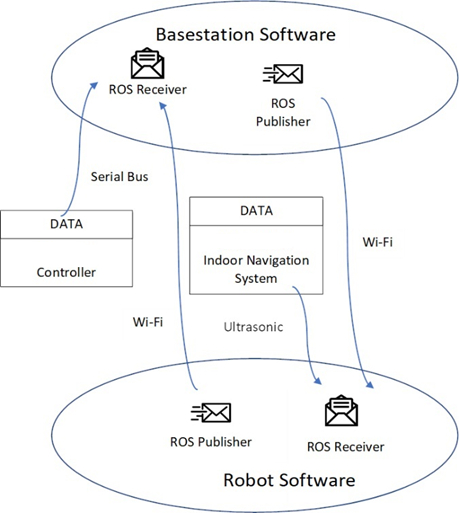
\includegraphics[width=0.53\textwidth]{software_arc.jpg}
    \end{center}
    \vspace{-20pt}
    \caption{The System Architecture}
    \vspace{-10pt}
  \end{wrapfigure}
There are two main software stacks, that of the
basestation and ORPS-Robot. The basestation
software will exist on a laptop, run a graphical user
interface for the user controlling the robot to
interact and control the robot via an Xbox 360
controller which will also be connected to this
basestation. This data will be fed to a ROS receiver
and be processed to be set to the ORPS-Robot. When
the user makes some change in the controller input
that is collected by the ROS receiver and fed through
the M-transformation to be received by the
single board computer on the robot via Wi-Fi. We have
not worked out what this position data will look like,
whether it be an actual video signal via a camera or
the positioning data via the LiDAR but there will be
some graphical user interface component to this project.\\\\
On the basestation as mentioned previously we will be publishing commands to the robot, including
the movement commands via the controller but also doing error measurements between what the user
commanded the robot to go and where it went. This is where the path smoothing part of the project
comes into play. There will be some desired position and an actual position of the robot. The actual
position will be what the Marvelmind ultrasonic indoor navigation system calculates and the desired
position will be where the system tells the user to go. The aim is to minimize the error between the
actual position and the desired position, even with latent inputs.\\\\
As for the software on the robot itself, it must be capable of receiving data from a Marvelmind sensor
which will be connected to the robot itself via USB 2.0. This positioning data will be processed on the
Marvelmind itself and will be published for further processing on the basestation. The robot software,
which will be running on a single board computer must be able to receive ROS commands from the basestation
and publish the position data to the basestation. As the communication delay is too great to be doing
this all on the basestation this means the system must be robust enough to be setup to run then process
the information it receives on its own. This also means controlling the microcontroller to
control the actuator motors on the robot itself for movement.
\begin{figure}
    \centerline{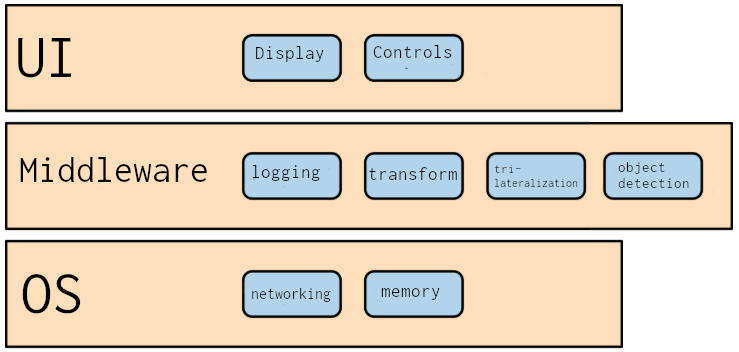
\includegraphics[scale = 2.5]{cake.jpeg}}
    \caption{Cake Diagram of the Software Architecture}
\end{figure}
\section{System Design}
For this project we need to produce a semiautonomous robot to aid in network control systems
research. A network control system is a spatially distributed system wherein the control loop is closed
through a communication network. This raises fundamental challenges and benefits to the overall 
system design. By closing our loop over some communication network, we can do some processing on
our laptop and some processing on the ORPS-Robot itself, allowing for a separation in system
components, that in aggregate work better and more cheaply than standalone systems.\\\\ 
The major challenges include unifying communication, estimation, control and control over networks. To send a
signal over a digital network, the signal must be sampled, encoded in some digital format, transmitted
over the network and finally the data must be decoded at the receiver side, which will induce large,
potentially intermittent delays in the feedback loop. The variable network conditions such as congestion
and channel quality may also induce variable delays between sampling and decoding at the receiver due
to network access delays. Whenever you are dealing with feedback, reducing delay times are a primary
for any linear time invariant system. It will be our job to reduce the delay and make it as stable as
possible. The key role of this section will be to articulate a design pattern which will most accurately and
acutely mitigate the limitations of network control systems.
\subsection{Hardware Design}
There are three levels to the ORPS robot. A bottom level where the chassis, motors, wheels and battery
exist. A middle section where the microcontroller exists and a top section with Raspberry Pi. On top of the robot
itself exists the LiDAR. The chassis are made of up waffle like plates, which allow for customization to
our preferences, which we may very well take advantage of. We are unsure whether we will use the
LiDAR or not on this system. Marvelmind is an ultrasonic local positioning system and be used as 
the mobile beaconing system.
\subsubsection{Objectives}
The hardware design for this project is largely preset, coming from the manufacturer already assembled.
In this respect our job is to finish this product, not design our own from scratch. There are tradeoffs and
benefits to this approach. One tradeoff is that we have less flexibility to choose overcome challenges
with hardware fixes, but the largest benefit is that it allows us to focus on delivering the product that
our client wants most, which is a platform for research. The bottom line is to get this done as quickly and
efficiently as possible, and that means taking what works off the shelf.
\subsubsection{Constraints}
I do not know what the constraints of our system are at this point or what should be in this
section.
\subsubsection{Composition}
\paragraph{Xbox 360 Controller}
The human interface device available is a commercial game controller. ROS has a node that can publish
the current controller state as a topic. This controller will be connected to the laptop Base station using
USB 2.0. The controller joysticks and triggers return an analog value to the laptop while the rest of the
buttons work as a digital on and off switch.
\paragraph{Marvelmind Indoor Navigation System}
Marvelmind indoor navigation system is designed for precise ($\pm 2 cm$) location data meant for
specifically off-the-shelf usage in autonomous robot, vehicle and copters. This product was chosen
mainly due to its accuracy, which is very important for our application as it involves control systems
based on position.
\paragraph{Raspberry Pi Model B}
Raspberry Pi is a small computer which we are using as our main controller on the ORPS-Robot. It will be
running Libuntu, and act as our point of contact to the ORPS-Robot. The Raspberry was chosen for this
project because of its small form factor, affordability, functionality, and because it was included in the
burger bot package that was purchased.\\\\
If we need more computing power to run the image recognition stretch goal, we could switch out this
board for something more powerful or outsource the processing to the laptop.
\paragraph{OpenCR}
OpenCR is a controller board used for controlling the different robotic components. This board is open
source and made specifically for working with ROS systems. This board is attached to the battery, which
it uses to supply power to all the other components on the robot. The OpenCR is programmable with
the Arduino software development environment meaning that in addition to using ROS to control the
ORPS-Robot, we have access to addition programming patterns using Arduino’s C/C++ functions and
libraries. The OpenCR board was included in the Burger bot from ROBOTIS.
\paragraph{DYNAMIXEL Actuator System}
The motors for the ORPS-Robot use DYNAMIXAL XL430-W250 motors. There is one motor for each of
the two wheels. The motor system was included in the Burger bot from ROBOTIS.
\paragraph{Li-Po Battery}
The battery on the ORPS-Robot is a Li-Po Battery with a power output of 12V DC, 5A. This battery is
connected to the OpenCR board where it is used to power the whole robot. This is a 18,000 mAh
battery. The battery was included in the ORPS-Robot.
\paragraph{LDS-01 LiDAR}
The LDS-01 is a 2D laser scanner capable of sensing $360\degree$ that collects a set of data around the ORPSRobot
to use for SLAM (Simultaneous Localization and Mapping) via a USB 2.0 connection on the
Raspberry Pi 3. This portion was excluded from the figures as it is not a crucial part of the hardware
architecture and may be excluded from the final revision.
\subsubsection{Interface}
\paragraph{Xbox 360 Controller}
The main controlling interface for the ORPS-Robot. This uses USB 2.0.
\paragraph{Marvelmind Indoor Navigation System}
The Marvelmind sensors are attached to the Raspberry Pi via USB 2.0.
\paragraph{Raspberry Pi 3 Model B}
The Raspberry Pi 3 will be connected to the laptop via Wi-fi, and the OpenCR and Marvelmind via USB.
The Pi is equipped with HDMI and USBs which we will use to run the programs we create.
\paragraph{OpenCR}
The OpenCR is connected to the Raspberry PI 3 via USB 2.0 and to the DYNAMIXAL Actuator system via
RS-485. The OpenCR also has many other interfaces which we do not currently have any plans to use.
\paragraph{DYNAMIXAL Actuator System}
The motors are connected to the OpenCR on a TTL Multidrop Bus using a TTL Half Duplex Asynchronous
Serial Communication protocol.
\paragraph{Li-Po Battery}
This battery is connected to the OpenCR using basic power connectors.
\subsection{Software Design}
This is mostly an embedded software project. There will be an embedded layer and host layer, where
the embedded layer is split into three separate layers. For now, it will be described with a table. For
future updates there will be a graphic that describes this. We need to meet as a group and hash out
what this exactly looks like all together.
\subsubsection{Objectives}
This project is predominately a software project, as such much of the objectives of the overall project 
are in this section itself. In this section we will lay out a sequence of steps for us to hit to have a 
finished product. The ability to control the robot, over a communication network, must be demonstrated 
then data must be collected on this action. Once those two things are demonstrated then the transformation 
algorithms will be implemented into the project. After this the GUI will be constructed for further 
testing and simulation.
\subsubsection{Constraints}
I do not know what the constraints of our system are at this point or what should be in this
section.
\subsubsection{Compositions}
\subsubsection{Uses and Interactions}
\subsubsection{Interface}
\subsubsection{Resources}
\subsubsection{Base Station Software}
\paragraph{Robot Operating System (ROS)}
ROS is a middleware library that creates interfaces for many common robot components and allows
them to communicate in standardized ways. Each ROS process is called a node. Nodes communicate
through topics or services. A service provides a classic server-client model where the client makes a
request and the server responds. A topic implements a logical many-to-many data bus. Nodes can
publish to or subscribe from any topic without knowing anything about other nodes on the topic.
\paragraph{Graphical User Interface (GUI)}
When in remote control mode the robot can be controlled by a consumer game controller. Ideally the
user will be presented with a graphic of a 2-dimensional field with a marker representing the robot’s 
current position and a fixed path to follow. The user will be tasked with attempting to make the robot
follow the displayed path.
\subsubsection{R-Transformation}
\begin{wrapfigure}{r}{0.5\textwidth}
    \vspace{-20pt}
    \begin{center}
      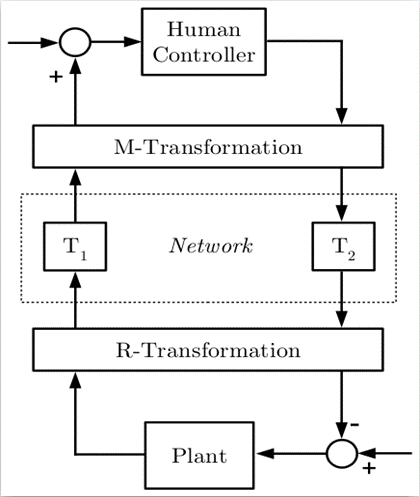
\includegraphics[width=0.48\textwidth]{ovr_tran.jpg}
    \end{center}
    \vspace{-20pt}
    \caption{The Overall Control Loop with Transformations}
    \vspace{-10pt}
  \end{wrapfigure}
The control signals from the Wi-Fi network will take the
form of a 1x2 integer vector indicating speed and
direction. As of this writing the actual math has not been
explained to us for the R-Transformation other than to
say this is more than a simple linear transformation,
requiring more operations than the M-Transform. Our job
is to test this functionality as a black box, not necessarily
understand it.
\subsubsection{M-Transformation}
The control signals from the human controller will take
the form of a 1x2 integer vector indicating speed and
direction. As of this writing the actual math has not been
explained to us for the M-Transformation other than to
say this is a simple linear transformation. Our job is to
test this functionality as a black box, not necessarily
understand it.
\subsubsection{Human Interface Design}
The ORPS-Robot must provide a graphical user interface
that provides some prompt on how to control the robot via
the controller or keyboard and how to read the commands. Good design is an act of communication.
The graphical user interface must be cognizant of the type of user that will use this device and able to be
operated by not only the creators of the ORPS-Robot but Michael McCourt and future researchers in this
area.
\section{Ethical Considerations}
In this project, our specific goals do not raise many ethical concerns, however, there are still things that
could happen from this project that should be considered.\\\\
The primary purpose of the algorithm being tested here is to help with the delay of
human interacting in closed loop control systems. This algorithm could be used for military systems or
other weapons systems. Control systems have social and ethical implications, mainly 
because of the sorts of products they are produced for. Control is a tool for mitigating 
uncertainty, and devices made to deal with such uncertainty are often employed in military settings 
or where users have a great deal of expectations out of the devices to work well under a broad swath 
of possible inputs to a system.\\\\
This project is funded by Dr. McCourt who has funding from the University of Washington. 
We did not technically earn this money, so it is our responsibility to use this money efficiently.
To help mitigate both ethical considerations a formulation of design requirements and criteria 
was established in this document, with an acceptance of tradeoffs between different design criteria 
was established outside of the document in team meetings. This design decisions in this document are 
the end results of such a process. 
\section{References}
\section{Errata}
\end{document}